%% ZKFL-PQ — IEEE conference manuscript (≤6 pages, dense)
%% PDF eXpress conference ID: 61911X
\documentclass[conference]{IEEEtran}

\usepackage{iftex}
\ifPDFTeX
  \usepackage[T1]{fontenc}
  \usepackage[utf8]{inputenc}
  \usepackage{times}
\else
  \usepackage{fontspec}
  \setmainfont{TimesNewRoman}[
    Path = ./fonts/, Extension = .ttf,
    UprightFont = times, BoldFont = timesbd,
    ItalicFont = timesi, BoldItalicFont = timesbi]
  \setmonofont{CourierNew}[
    Path = ./fonts/, Extension = .ttf,
    UprightFont = cour, BoldFont = courbd,
    ItalicFont = couri, BoldItalicFont = courbi]
\fi

\usepackage{cite}
\usepackage{amsmath,amssymb,amsfonts,amsthm,mathtools}
\usepackage{algorithm}
\usepackage{algpseudocode}
\usepackage{graphicx}
\usepackage{booktabs}
\usepackage{url}
\usepackage{balance}
\usepackage{microtype}
\usepackage{enumitem}
\usepackage{multirow}

\newtheorem{theorem}{Theorem}
\newtheorem{definition}{Definition}
\newtheorem{remark}{Remark}

\newcommand{\norm}[1]{\lVert #1 \rVert}
\newcommand{\Enc}{\mathsf{Enc}}
\newcommand{\Dec}{\mathsf{Dec}}
\newcommand{\Prove}{\mathsf{Prove}}
\newcommand{\Verify}{\mathsf{Verify}}
\newcommand{\Commit}{\mathsf{Commit}}

\usepackage[
  letterpaper, top=0.88in, bottom=1.15in,
  left=0.68in, right=0.68in, columnsep=0.2in,
  noheadfoot, nomarginpar
]{geometry}
\pagestyle{empty}
\markboth{}{}

\begin{document}

\title{Zero-Knowledge Federated Learning with Lattice-Based Hybrid Encryption for Quantum-Resilient Medical AI}

\author{
\IEEEauthorblockN{Edouard Lansiaux}
\IEEEauthorblockA{STaR-AI \& Emergency Department, CHU de Lille, Lille, France\\
Email: edouard1.lansiaux@chu-lille.fr}
}

\maketitle
\thispagestyle{empty}

\begin{abstract}
Hospital federated learning (FL) must resist gradient inversion, Byzantine poisoning, and Harvest-Now-Decrypt-Later (HNDL) risk under multi-year retention. \textbf{ZKFL-PQ} is a \emph{compositional} stack---not a single new primitive---engineered so each hospital threat maps to an explicit layer: NIST ML-KEM-768 transport; dual-norm language $\mathcal{L}_{\tau_2,\tau_\infty}^{\mathrm{bind}}$ (Unruh $\ell_2$ NIZK + public $\ell_\infty$ clip on the \emph{same} BFV plaintext); Unruh-lifted Enc-consistency; $(t,n)$-threshold BFV open with a PartialDecrypt FS accountability check; adaptive public $\tau_2$ and round-transcript binding; and default post-ZKP median. The artifact ships fused SEAL+threshold HE, shared-SIS Unruh, Keccak/SHA3 formal checks, and measured demos with explicit library-default vs.\ latency $r$. Empirically we report 5-seed synthetic baselines, UCI pipeline validation under the innovation stack, MedMNIST/\texttt{ConvNet28} smokes, backdoor ASR, and a sparse-poison dual-norm ablation ($100\%$ reject vs.\ $0\%$ for $\ell_2$-only). Complementary to Beskar-class secure aggregation---not a replacement.
\end{abstract}

\begin{IEEEkeywords}
Post-quantum cryptography, federated learning, zero-knowledge proofs, homomorphic encryption, medical AI, Byzantine robustness
\end{IEEEkeywords}

\section{Introduction}
Federated learning (FL)~\cite{mcmahan2017fedavg} keeps raw records at the edge, yet model updates remain vulnerable to gradient inversion~\cite{zhu2019deep}, Byzantine poisoning~\cite{blanchard2017machine}, and HNDL attacks against classical TLS when medical archives outlive RSA/ECC~\cite{mosca2018cybersecurity}. Hospital consortia therefore need (i)~post-quantum (PQ) session confidentiality, (ii)~verifiable rejection of oversized updates, and (iii)~aggregation that does not place a single curious server in sole possession of plaintext gradients.

Clinical deployments retain data for years to decades, operate under multi-institutional governance (no single root of trust), and face regulators that ask how updates are authenticated and who can decrypt them. Wrapping FedAvg in classical TLS is insufficient against adversaries that store ciphertexts today and open them later~\cite{mosca2018cybersecurity}. Cryptographic accept alone is also insufficient: updates whose $\ell_2$ norm respects a public threshold $\tau$ can still flip signs or implant triggers, so statistical robust aggregation must follow a successful proof. Conversely, robust aggregation alone does not provide PQ transit, ciphertext binding, or multi-party decrypt---hence the need for an explicitly layered stack.

\paragraph{Design goals.}
We optimize for hospital consortia where (G1)~ciphertext retention is measured in years, (G2)~no single IT operator may hold a usable $sk$, (G3)~oversized gradients must be rejectable without trusting the client, (G4)~sparse $\ell_\infty$ spikes that pass an $\ell_2$ gate must be rejectable before opening, and (G5)~in-bound Byzantine behavior that still satisfies $(\tau_2,\tau_\infty)$ is handled by a robust aggregator rather than by tightening $\tau$ until honest sites fail.

\paragraph{Why composition is the contribution.}
Each goal is already partially addressed by known tools (ML-KEM, lattice Σ-protocols, BFV, median/Krum, Unruh). The scientific gap for medical PQ-FL is \emph{binding}: a proof that is accepted must refer to the same plaintext that is encrypted; a threshold open must reject a malformed partial; demo parameters must not be silently inflated into 128-bit claims; and $\ell_2$ gates must not be sold as backdoor-complete. ZKFL-PQ's novelty is therefore the dual-norm language, Unruh-uniform Enc-consistency, PartialDecrypt accountability, adaptive/transcripted thresholds, and the empirical separation of cryptographic vs.\ statistical metrics (Tables~\ref{tab:threats},~\ref{tab:res},~\ref{tab:dual}).

\paragraph{Contributions.}
\begin{enumerate}[leftmargin=*,nosep]
  \item A layered protocol for $\mathcal{L}_{\tau_2,\tau_\infty}^{\mathrm{bind}}$ with Unruh Enc-consistency, PartialDecrypt-accountable threshold open, then post-ZKP median (Table~\ref{tab:threats}, Algorithm~\ref{alg:target}).
  \item Dual-norm gating, adaptive public $\tau_2$, and transcript binding---with honest scope on which gadgets are Unruh vs.\ classical FS.
  \item Concrete parameters (library defaults vs.\ latency demos), an \emph{informal} composition theorem with explicit assumptions, Lean/Python/EasyCrypt checks, and measured payloads/latency.
  \item A reproducible artifact~\cite{zkflcode} and empirical study: multi-seed baselines, innovation-pack UCI pipeline validation, MedMNIST/\texttt{ConvNet28} smokes, backdoor ASR, and dual-norm ablation (Table~\ref{tab:dual}).
\end{enumerate}

\section{Threat Model and Claims}
\textbf{Adversary:} (i)~a network eavesdropper with future quantum computers against factoring/DLP; (ii)~up to $f{<}N/2$ Byzantine clients that may submit arbitrary vectors and proofs; (iii)~a curious aggregator that sees all protocol messages but does not hold $sk$ alone; (iv)~up to $t{-}1$ colluding threshold decryptors, \emph{plus} one decryptor that may return a malformed partial $\mu_i$ (open must abort rather than silently bias).

\textbf{Trust.} Honest clients follow local SGD, $\ell_\infty$ clipping, and Prove. Honest decryptors compute $\mu_i$ correctly. The aggregator runs $\Verify$ and the chosen robust aggregator correctly, but is not trusted for confidentiality of individual updates once shares are distributed.

\textbf{Claims:} ML-KEM-768 transport (FIPS~203 Level~3)~\cite{nist_fips203_2024}; dual-norm membership in $\mathcal{L}_{\tau_2,\tau_\infty}^{\mathrm{bind}}$ under SIS+Unruh/RO for the $\ell_2$ sessions and clip+Enc-consistency binding for $\ell_\infty$; Unruh Enc-consistency against proof/ct splits; threshold privacy and open abort against a malicious partial (PartialDecrypt FS, ROM); transcript non-swap across rounds via $H_{t-1}$.

\textbf{Scope.} We do not claim differential privacy, clinical efficacy from UCI/MedMNIST pipeline runs, HomomorphicEncryption.org certification of the NumPy $n{=}512$ demo preset, or a drop-in replacement for Beskar-class full-stack secure aggregation~\cite{zhang2025beskar}. Pure $\ell_2$ alone does not stop sign-flip or diffuse in-bound backdoors (Tables~\ref{tab:threats},~\ref{tab:res}).

\begin{table}[t]
\caption{Threat coverage by layer (composition is the contribution).}
\label{tab:threats}
\centering
\scriptsize
\begin{tabular}{@{}lccccc@{}}
\toprule
Threat & ML-KEM & Dual-norm & Unruh-Enc & PD-NIZK & Median \\
\midrule
HNDL / PQ transit & yes & -- & -- & -- & -- \\
Oversized update & -- & $\ell_2$ & -- & -- & -- \\
Sparse / $\ell_\infty$ spike & -- & $\ell_\infty$ & -- & -- & help \\
Proof/ct split & -- & bind & yes & -- & -- \\
Malicious partial $\mu_i$ & -- & -- & -- & abort & -- \\
Curious aggregator & -- & -- & -- & thr. & -- \\
Sign-flip / backdoor & -- & no$^{\ddagger}$ & -- & -- & yes \\
\bottomrule
\end{tabular}\\[1pt]
{\footnotesize $^{\ddagger}$In-bound updates may still satisfy $(\tau_2,\tau_\infty)$; Table~\ref{tab:res}: 0\% crypto detection for sign-flip under $\ell_2$ alone.}
\end{table}

\section{Related Work}
\begin{table}[t]
\caption{Positioning vs.\ related PQ / robust FL lines.}
\label{tab:rel}
\centering
\scriptsize
\begin{tabular}{@{}lccc@{}}
\toprule
System & PQ transport & Norm ZKP & HE / thr.\ dec. \\
\midrule
Beskar~\cite{zhang2025beskar} & yes (masking/DP) & -- & secure agg.\ stack \\
Patel~\cite{patel2025pqfl} & lattice HE & -- & HE FL \\
Lu et al.~\cite{lu2024hybrid} & hybrid PQ & -- & HE FL \\
Krum~\cite{blanchard2017machine} & -- & statistical & -- \\
zkML~\cite{kang2022zkml} & -- & inference ZK & -- \\
ZKFL-PQ (ours) & ML-KEM-768 & Unruh+bind & BFV$(t,n)$+PD \\
\bottomrule
\end{tabular}
\end{table}

Beskar offers a mature PQ secure-aggregation stack with assisting nodes and DP~\cite{zhang2025beskar}. Patel~\cite{patel2025pqfl} and Lu et~al.~\cite{lu2024hybrid} study PQ-HE FL without ciphertext-bound norm ZKPs. zkML targets inference proofs rather than FL aggregation~\cite{kang2022zkml}. Classical robust aggregators (Multi-Krum, coordinate median, trimmed mean) remain effective against low-norm adversaries but do not provide PQ transport, ciphertext binding, or threshold open correctness. ZKFL-PQ therefore \emph{composes} cryptographic accept with median/Krum rather than replacing either line: Hybrid+mean vs.\ Hybrid+median (Table~\ref{tab:res}) and dual-norm vs.\ $\ell_2$-only (Table~\ref{tab:dual}) make the division of labor measurable. We intentionally avoid claiming superiority over Beskar; the stacks are complementary (masking/DP vs.\ ct-bound Unruh+threshold open).

\section{Protocol Design}

\subsection{Round Structure}
Each round $t$: the server broadcasts $w^{(t)}$, public $(\tau_2,\tau_\infty)$, and transcript hash $H_{t-1}$. Client $i$ runs local SGD, applies $\mathrm{Clip}_\infty$ then quantization into $\tilde{w}_i\in\mathcal{L}_{\tau_2,\tau_\infty}^{\mathrm{bind}}$, encrypts under BFV $pk$, produces Unruh Enc-consistency and Unruh norm proofs bound to $\mathbf{ct}_i$, and sends an ML-KEM-wrapped payload. The server verifies, threshold-opens with PartialDecrypt NIZK (abort on malice), applies coordinate-wise median, then publishes adapted $\tau_2$ and $H_t$ (Algorithm~\ref{alg:target}).

\paragraph{Transport.}
ML-KEM-768 encapsulates a session key used to AES-CTR-wrap $(\mathbf{ct}_i,\pi_i,\pi_i^{\mathrm{enc}})$. This protects in-transit confidentiality against classical and future quantum adversaries on the channel; it does not replace HE confidentiality against the aggregator, which follows from RLWE + threshold opening.

\paragraph{Verification checklist.}
$\Verify$ returns $1$ iff: (i)~Unruh invertible-RO records are consistent for the norm proof; (ii)~challenge bits match the recomputed digest of first messages, $\mathbf{ct}_i$, public $(\tau_2,\tau_\infty)$, and $H_{t-1}$; (iii)~SIS algebraic checks hold against the shared $\mathbf{A}$; (iv)~response $\ell_2$ norms respect $B$ and Enc-consistency attests the same plaintext obeys the public $\ell_\infty$ clip; (v)~Unruh Enc-consistency accepts for every BFV chunk. Fail-closed: any failed check drops the client for that round.

\subsection{Quantization, Dual-Norm, and Adaptive $\tau_2$}
$\mathrm{Quantize}$ clips to $[-c,c]$, scales by $s$, and rounds into $\mathbb{Z}_t$ (defaults $c{=}1$, $s{=}10^{3}$). Honest clients set $\tilde{w}\leftarrow\mathrm{Clip}_\infty(\mathrm{Quantize}(\Delta),\tau_\infty)$ and prove $\norm{\tilde{w}}_2\le\tau_2$ on that same vector. Sparse spikes with $\norm{\cdot}_2\le\tau_2$ but $\norm{\cdot}_\infty>\tau_\infty$ are rejected before opening; Enc-consistency prevents proving a clipped vector while encrypting an unclipped one.

Adaptive public $\tau_2$ uses an EMA of a high quantile of accepted norms:
\begin{equation}
\tau_2^{(t+1)}=\mathrm{clip}\!\left((1-\beta)\tau_2^{(t)}+\beta\cdot \gamma\, Q_{1-\alpha}(\{\norm{\Delta_i}\}_{i\in S_t}),[\tau_{\min},\tau_{\max}]\right),
\end{equation}
with defaults $\alpha{=}0.1$, $\gamma{=}1.25$, $\beta{=}0.5$ in the artifact. Both $\tau_2^{(t)}$ and $H_{t-1}$ enter the Unruh associated data, so clients cannot silently ignore the published schedule.

\subsection{Bound Dual-Norm Language}
\begin{definition}[Dual-norm bound language]
Let $C=\Commit(\tilde{w};\mathbf{r})=\mathbf{A}(\tilde{w}\|\mathbf{r})\bmod q'$,
$\mathbf{ct}=\Enc_{pk}(\tilde{w};\rho)$, and public $(\tau_2,\tau_\infty)$. Then
\begin{multline}
\mathcal{L}_{\tau_2,\tau_\infty}^{\mathrm{bind}}=
\bigl\{(C,\mathbf{ct},\tau_2,\tau_\infty):\exists(\tilde{w},\mathbf{r},\rho)\\
\quad C=\Commit(\tilde{w};\mathbf{r}),\
\mathbf{ct}=\Enc(\tilde{w};\rho),\\
\quad \norm{\tilde{w}}_2\le\tau_2,\
\norm{\tilde{w}}_\infty\le\tau_\infty\bigr\}.
\end{multline}
\end{definition}

\begin{remark}[What is Unruh vs.\ policy]
The $\ell_2$ predicate is enforced by Unruh parallel sessions. The $\ell_\infty$ predicate is enforced by the public clip \emph{plus} Enc-consistency binding that plaintext to $\mathbf{ct}$---not by a separate Unruh range proof. This is intentional: it is efficient at imaging-scale $d$ and still closes the sparse-spike attack of Table~\ref{tab:dual}.
\end{remark}

\paragraph{$\Sigma$-protocol~\cite{lyubashevsky2012lattice}.}
Commit masks $\mathbf{y}$ and message $\tilde{w}$; responses $(\mathbf{z},\mathbf{r}_z)$ satisfy $T+eC\equiv\mathbf{A}(\mathbf{z}\|\mathbf{r}_z)$ and $\norm{\mathbf{z}}_2\le B$. Rejection sampling yields HVZK in the classical ROM. Acceptance uses only algebraic and norm checks---never a client-supplied Boolean.

\paragraph{Unruh-oriented NIZK.}
Classical FS is not tightly QROM-secure~\cite{kiltz2018qrom}. We use parallel binary Unruh sessions (library default $r{=}128$; latency demos $4$--$64$) with invertible-RO records $(\rho,H(\rho))$. Challenge bits come from $H(\mathsf{UNRUH}\|\tau_2\|\tau_\infty\|H_{t-1}\|\mathbf{ct}\|\mathsf{first\text{-}msgs})$. All sessions share one SIS matrix $\mathbf{A}$ (shape $256{\times}(d{+}128)$), avoiding $r$ independent keys at large $d$. Lean~4 checks combinatorial uniqueness/$2^{-r}$; EasyCrypt ships SHA3/Keccak lane theories with executable FIPS checks (\texttt{formal/run\_formal\_ci.py}).

\paragraph{Enc-consistency (Unruh-lifted).}
A Σ-gadget proves knowledge of coins $\rho=(u,e_0,e_1)$ s.t.\ the BFV equations hold for the encrypted plaintext chunk. We lift it under the same Unruh transform as the norm proof (binary sessions + invertible RO), closing the QROM-uniformity residual between the two ct-bound gadgets. First messages are absorbed into the norm proof's associated data.

\subsection{BFV Aggregation and Threshold Opening}
\begin{table}[t]
\caption{Cryptographic parameters (research stack).}
\label{tab:params}
\centering
\scriptsize
\begin{tabular}{@{}llp{0.42\columnwidth}@{}}
\toprule
Component & Setting & Notes \\
\midrule
ML-KEM-768 & $n{=}256,k{=}3,q{=}3329$ & FIPS~203 L3~\cite{nist_fips203_2024} \\
BFV degree & $n{=}512$ / $4096$ & Demo vs.\ \texttt{classic128} preset \\
BFV moduli & $q{\approx}2^{40}$, $t{=}2^{12}$ & Research NumPy encoder \\
Threshold & $(2,3)$ partial decrypt & Server $sk{=}\bot$ \\
Unruh $r$ & $128$ library default & Demos may use $16$--$64$ \\
Enc-Unruh $r_{\mathrm{enc}}$ & parallel / chunk & Latency demos use $4$--$8$ \\
Dual-norm & $\tau_2$+$\tau_\infty$ & Same Prove+Enc vector \\
Open audit & PartialDecrypt FS & Abort on bad $\mu_i$ \\
SIS $\mathbf{A}$ & shared $256{\times}(d{+}128)$ & Not $r$ copies \\
\bottomrule
\end{tabular}
\end{table}

Additive BFV yields $\Dec(\sum_i\Enc(m_i))=\sum_i m_i$ under noise growing roughly as $N\cdot O(\sigma\sqrt{n})$. Full-vector packing encrypts all $d$ coordinates as $\lceil d/n\rceil$ ciphertexts; the ZKP covers the concatenated vector (no unprotected suffix). After keygen, $sk$ is Shamir-shared and erased. Party $i$ returns $\mu_i=c_1\star(\lambda_i\cdot s_i)$ plus smudging. PartialDecrypt NIZK proves knowledge of $s_{\mathrm{eff}}$ with $\mu_i=c_1\star s_{\mathrm{eff}}$ under FS (ROM): if $\mu_i$ is tampered, verify fails and the open aborts. Modular negacyclic mul with parallel per-chunk encrypt keeps $d{\approx}5{\times}10^{4}$ interactive on CPU. Optional \texttt{FusedSealThresholdHE} runs a TenSEAL sidecar beside threshold open.

\paragraph{Post-ZKP aggregation.}
For accepted set $S$, default $\bar{\Delta}_j=\mathrm{med}\{\Delta_{i,j}:i\in S\}$. Multi-Krum and mean are overrides. Median is applied \emph{after} cryptographic accept: it does not replace the ZKP, and the ZKP does not replace median.

\begin{algorithm}[t]
\caption{ZKFL-PQ round (innovation composition)}
\label{alg:target}
\begin{algorithmic}[1]
\Require $w^{(t)}$, $(\tau_2,\tau_\infty)$, KEM keys, HE $pk$, decryptor shares, $H_{t-1}$
\State Broadcast $w^{(t)}$, $(\tau_2,\tau_\infty)$, $H_{t-1}$
\For{each client $i$}
  \State $\tilde{w}\gets\mathrm{Clip}_\infty(\mathrm{Quantize}(\mathrm{LocalSGD}(w^{(t)},D_i)),\tau_\infty)$
  \State $\mathbf{ct}_i\gets\Enc_{pk}(\tilde{w};\rho_i)$; $\pi_i^{\mathrm{enc}}\gets\mathrm{UnruhEnc}(\rho_i)$
  \State $\pi_i\gets\Prove_{\mathrm{Unruh}}((\mathbf{ct}_i,\tau_2,\tau_\infty,H_{t-1}),\tilde{w})$
  \State send ML-KEM-wrapped $(\mathbf{ct}_i,\pi_i,\pi_i^{\mathrm{enc}})$
\EndFor
\State Keep $i$ iff dual-norm cryptographic verify returns $1$
\State For each accepted $i$: threshold-open with PartialDecrypt NIZK (abort if fail)
\State $\bar{\Delta}\gets\mathrm{Median}(\{\Delta_i\})$; publish $\tau_2\!\leftarrow\!\mathrm{Adapt}(\{\norm{\Delta_i}\})$, $H_t$
\State $w^{(t+1)}\gets w^{(t)}+\bar{\Delta}$
\end{algorithmic}
\end{algorithm}

\begin{theorem}[Informal composition]
Under SIS binding of $\Commit$, RLWE security of BFV, and RO modeling of $H{=}\mathsf{SHA3\text{-}256}$: (i)~honest members of $\mathcal{L}_{\tau_2,\tau_\infty}^{\mathrm{bind}}$ are accepted except for rejection-sampling aborts; (ii)~$\ell_2$-oversized witnesses are rejected except with Unruh/SIS advantage, while $\ell_\infty$ violations are rejected via clip+Enc-consistency binding (not a separate Unruh range proof); (iii)~Unruh Enc-consistency prevents proof/ct splits; (iv)~$t{-}1$ decryptors learn nothing beyond $t$ opens, and a malformed $\mu_i$ fails PartialDecrypt FS (ROM) and aborts; (v)~$H_{t-1}$ binds transcripts across rounds. Lean checks combinatorial $2^{-r}$ Unruh counting; EasyCrypt ships SHA3/Keccak with FIPS executable checks---not a fully discharged end-to-end EasyCrypt proof of the FL protocol.
\end{theorem}

\paragraph{Soundness sketch (Reviewer-A clarity).}
For binary Unruh with $r$ sessions, a cheating prover who can answer only challenge $0$ on an oversized witness is caught whenever a bit-$1$ challenge appears; the combinatorial counting lemma gives advantage $\approx 2^{-r}$ plus SIS forgery advantage on the commitment. Enc-consistency Unruh applies the same counting argument to the encryption coins. PartialDecrypt remains a classical FS relation proof $\mu=c_1\star s_{\mathrm{eff}}$; we mark it ROM and treat Unruh-lifting it as future work rather than silently claiming QROM uniformity for every gadget.

\paragraph{Implementation invariants and parameter honesty.}
The artifact~\cite{zkflcode} realizes Algorithm~\ref{alg:target} with shared prove/encrypt dimension, crypto-only accept, full-vector packing, Unruh Enc-consistency, PartialDecrypt open, fused SEAL+threshold HE, default median, shared SIS $\mathbf{A}$, adaptive $\tau_2$, and transcript binding. Library defaults: norm $r{=}128$, HE preset \texttt{classic128\_demo} ($n{=}512$). The innovation-pack demo uses $r{=}16$, $r_{\mathrm{enc}}{=}4$ for laptop CPU budgets and must not be quoted as the 128-bit Unruh class. Preset \texttt{classic128} ($n{=}4096$) is available and slower on NumPy; it is a parameter class, not a certified HomomorphicEncryption.org claim for the research encoder.

\section{Evaluation}

\subsection{Synthetic Multi-Baseline Study}
\textbf{Setup.} Synthetic 4-class task (1{,}000 samples, 784 features, Dirichlet $\alpha{=}0.5$), $N{=}5$, MLP with $d{=}108{,}996$, 10 rounds, seeds $\{42,\ldots,46\}$. Attacks from round~4: (i)~large-norm Gaussian; (ii)~sign-flip scaled to $\norm{\cdot}_2=\tau$. Baselines: FedAvg, clip@$\tau$, Multi-Krum ($f{=}1$), HE-only, ZKP-only, Hybrid+mean, Hybrid+median. Metrics: final accuracy (mean$\pm$std) and cryptographic detection rate.

\begin{table}[t]
\caption{Mean$\pm$std over 5 seeds (synthetic). Accuracy (\%) and detection.}
\label{tab:res}
\centering
\scriptsize
\begin{tabular}{@{}lcccc@{}}
\toprule
Method & Acc.\ (large) & Acc.\ (flip) & Det.\ (large) & Det.\ (flip) \\
\midrule
FedAvg & $26.0{\pm}1.0$ & $41.0{\pm}13.2$ & 0\% & 0\% \\
Clip@$\tau$ & $100{\pm}0$ & $40.3{\pm}12.7$ & -- & -- \\
Multi-Krum & $100{\pm}0$ & $100{\pm}0$ & -- & -- \\
HE-only & $22.1{\pm}2.1$ & $19.8{\pm}9.5$ & 0\% & 0\% \\
ZKP-only & $84.9{\pm}30.2$ & $40.9{\pm}13.2$ & 97\% & 0\%$^{\ddagger}$ \\
Hybrid+mean & $87.0{\pm}26.0$ & $40.1{\pm}12.6$ & 97\% & 0\%$^{\ddagger}$ \\
Hybrid+median & $100{\pm}0$ & $100{\pm}0$ & 97\% & 0\%$^{\ddagger}$ \\
\bottomrule
\end{tabular}\\[1pt]
{\footnotesize $^{\ddagger}$Sign-flip respects $\tau$---$\ell_2$ must accept. Hybrid+mean keeps plaintext mean after accept; Hybrid+median restores accuracy~\cite{zkflcode}.}
\end{table}

\begin{figure}[t]
\centering

\includegraphics[width=0.92\columnwidth]{figures/fig1_accuracy.png}
\caption{Synthetic accuracy under large-norm activation (seed~42).}
\label{fig:acc}
\end{figure}

\begin{figure}[t]
\centering
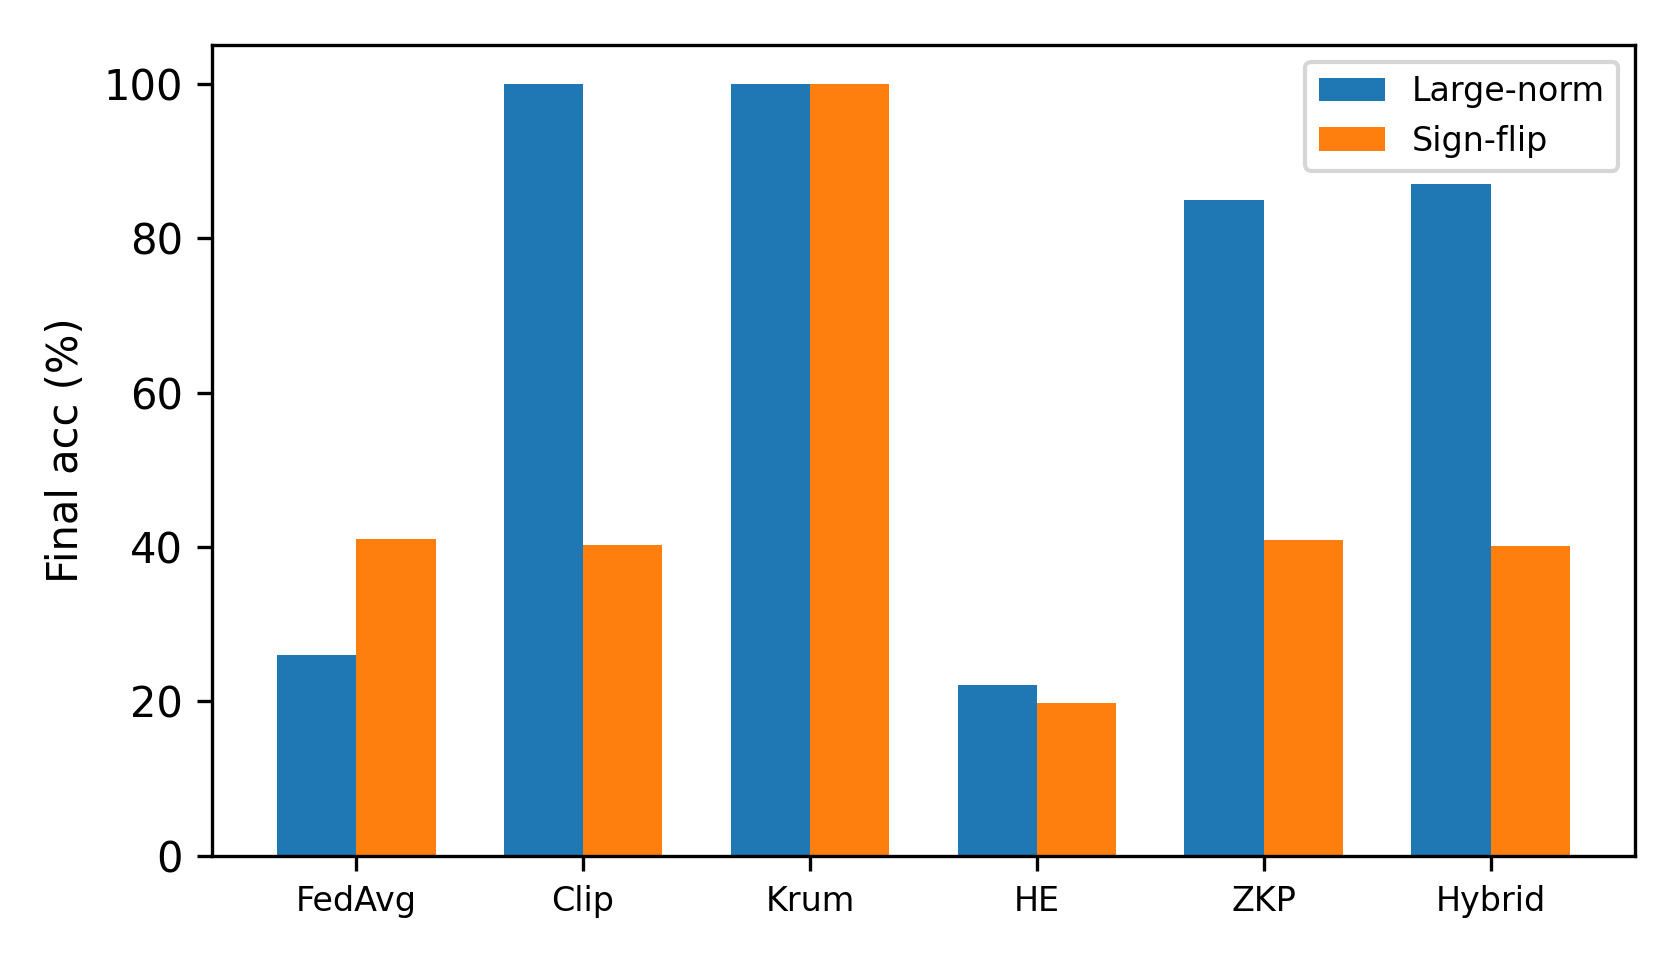
\includegraphics[width=0.92\columnwidth]{figures/fig_attacks.png}
\caption{Final accuracy: large-norm vs.\ sign-flip (5-seed means).}
\label{fig:att}
\end{figure}

Large-norm poisoning collapses FedAvg/HE-only; clipping, Multi-Krum, and ZKP-style filters retain accuracy (Table~\ref{tab:res}, Fig.~\ref{fig:acc}--\ref{fig:att}). Sign-flip within $\tau$ is accepted by pure $\ell_2$ and Hybrid+mean (0\% crypto detection), while Multi-Krum and Hybrid+median recover accuracy after cryptographic accept. The Hybrid+mean vs.\ Hybrid+median contrast is the empirical punchline for composition: privacy-preserving open without robust aggregation still fails on in-bound flips.

\paragraph{Takeaway (Reviewer B).}
Cryptographic detection is the right metric for oversized attacks; final accuracy after robust aggregation is the right metric for in-bound attacks. Reporting only one understates Table~\ref{tab:threats}. High variance on ZKP-only/Hybrid+mean large-norm accuracy ($84.9{\pm}30.2$, $87.0{\pm}26.0$) further motivates default median after accept.

\subsection{Scale, Medical Pipeline, Dual-Norm, and Backdoors}
A compact-model scale study with $N{=}20$, $T{=}30$ reproduces the same qualitative pattern: ZKP/hybrid reject oversized updates; sign-flip still needs robust aggregation.

On UCI Breast Cancer Wisconsin (569 samples, 30 features; MLP $d{=}1554$) we claim \emph{pipeline validation}, not clinical efficacy. The innovation stack (norm Unruh $r{=}16$, Enc Unruh $r_{\mathrm{enc}}{=}4$, PartialDecrypt NIZK, adaptive $\tau_2$, transcript, $\ell_\infty$ clip, threshold HE, median) yields $89.5\%\!\rightarrow\!93.0\%\!\rightarrow\!92.1\%$ over three rounds, rejects the oversized client, and adapts $\tau_2\!:\!8\!\rightarrow\!4.3\!\rightarrow\!2.3\!\rightarrow\!2.0$ ($\approx$20--23\,s/round; \texttt{innovation\_pack\_results.json}). Table~\ref{tab:dual} isolates the dual-norm gate. PneumoniaMNIST/\texttt{ConvNet28} ($\approx$51.6k params, no compact head) is an imaging smoke ($\approx$93.3\%, $r{=}4$) showing shared-SIS Unruh and modular BFV remain interactive before SGD dominates.

\begin{table}[t]
\caption{Sparse-poison ablation: $\norm{\cdot}_2\le\tau_2$ but $\norm{\cdot}_\infty>\tau_\infty$.}
\label{tab:dual}
\centering
\scriptsize
\begin{tabular}{@{}lcc@{}}
\toprule
Gate & Reject rate & Mean $|\mathrm{agg}_0|$ \\
\midrule
$\ell_2$-only & $0\%$ & $0.899$ \\
Dual-norm $(\tau_2,\tau_\infty)$ & $100\%$ & $0.003$ \\
\bottomrule
\end{tabular}\\[1pt]
{\footnotesize $\approx$265$\times$ spike reduction (\texttt{innovation\_pack\_results.json}).}
\end{table}

Trigger backdoors inside $(\tau_2,\tau_\infty)$ remain only partially mitigated by median (ASR $\approx$55\% vs.\ $\approx$98\% for FedAvg/$\ell_2$; Fig.~\ref{fig:bd}). Dual-norm removes sparse spikes \emph{before} opening; residual ASR is an honest limitation motivating DP/stronger aggregators (Beskar-complementary).

\begin{figure}[t]
\centering
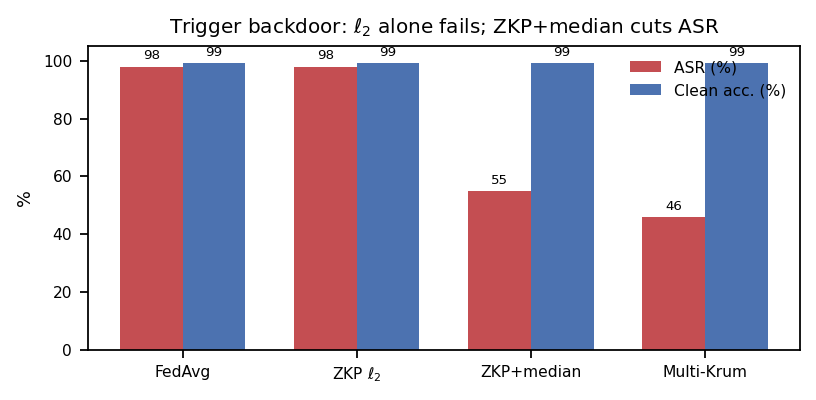
\includegraphics[width=0.92\columnwidth]{figures/fig_backdoor_asr.png}
\caption{Backdoor ASR vs.\ clean accuracy under FedAvg, $\ell_2$-ZKP, ZKP+median, and Multi-Krum.}
\label{fig:bd}
\end{figure}

\begin{figure}[t]
\centering
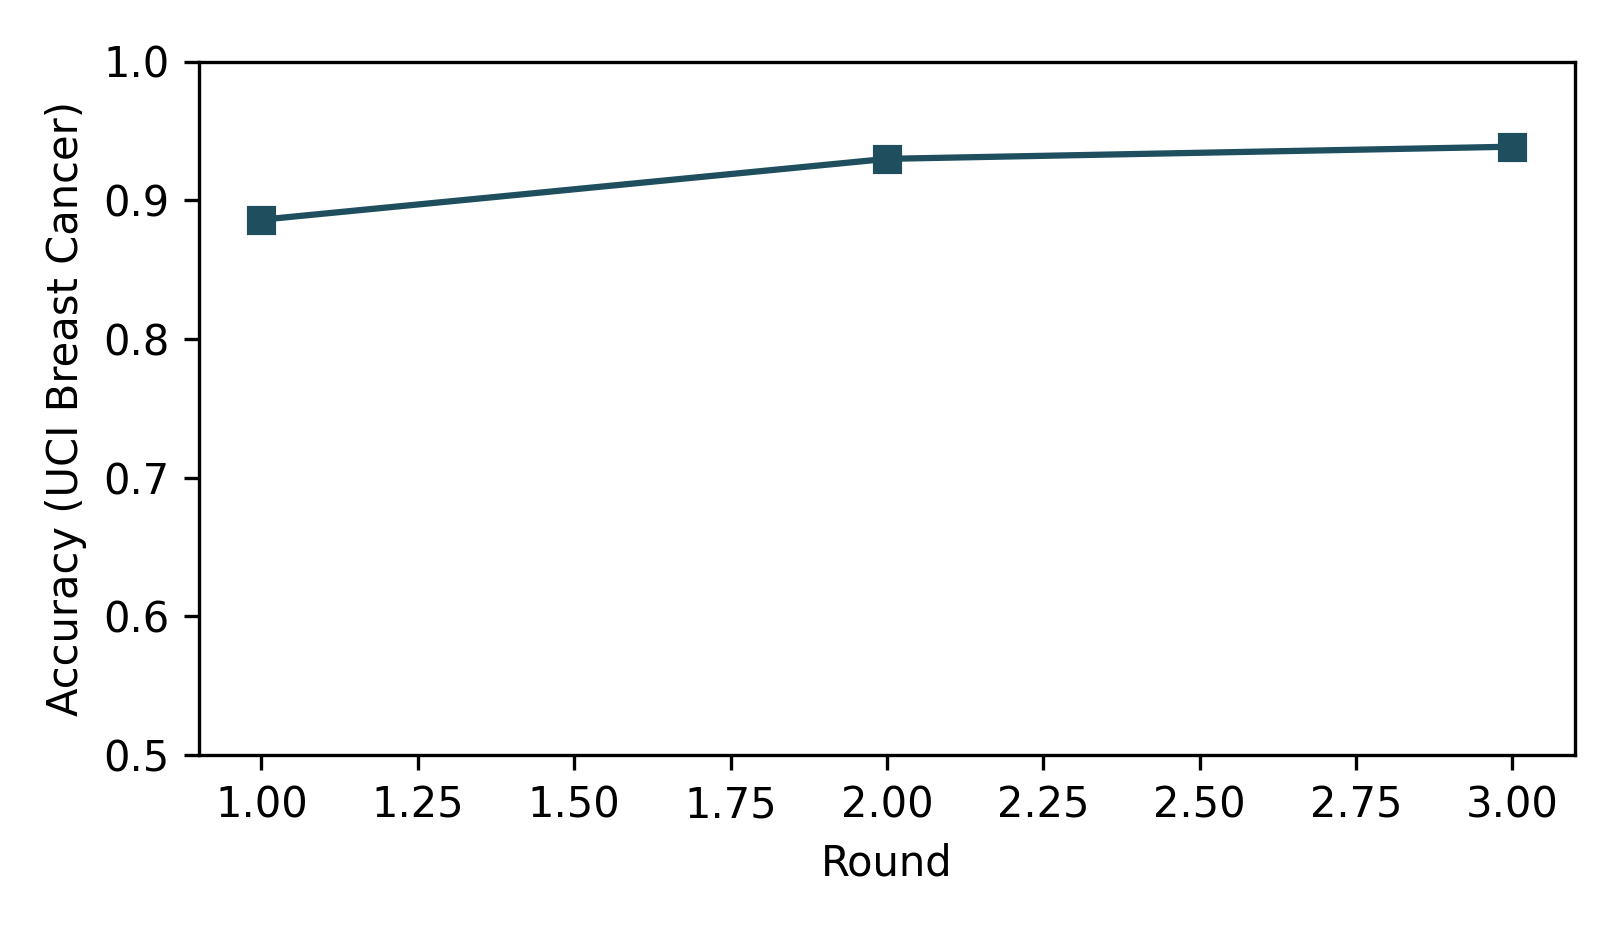
\includegraphics[width=0.92\columnwidth]{figures/fig_medical.png}
\caption{UCI Breast Cancer accuracy under the target/innovation pipeline.}
\label{fig:med}
\end{figure}

\begin{figure}[t]
\centering

\includegraphics[width=0.88\columnwidth]{figures/fig6_breakdown.png}
\caption{Mean round time (synthetic hybrid $\sim$20$\times$ FedAvg).}
\label{fig:break}
\end{figure}

\subsection{Communication and Latency Accounting}
\begin{table}[t]
\caption{Payload / latency (artifact; demo $r$ may be $<$ library default).}
\label{tab:comm}
\centering
\scriptsize
\begin{tabular}{@{}lcc@{}}
\toprule
Setting & Msg or time & Notes \\
\midrule
Synthetic hybrid & $\sim$100\,KB & Reference accounting \\
UCI target ($r{=}64$, $n{=}512$) & $\approx$4.7--5.9\,MB & Legacy target JSON \\
UCI innovation pack & $\approx$20--23\,s/round & Unruh-Enc+$\!$PD-NIZK \\
\texttt{ConvNet28} ($r{=}4$) & $\approx$2.4\,MB & $d{\approx}51.6$k \\
HE $n{=}4096$ preset & $\approx$2$\times$ ct vs $n{=}512$ & Slower on NumPy \\
\bottomrule
\end{tabular}
\end{table}
Uplink scales as $O\!\left(N\lceil d/n\rceil n\log q\right)$ plus Unruh $O(r(d+\ell))$ and Enc-Unruh $O(r_{\mathrm{enc}}\lceil d/n\rceil)$. Table~\ref{tab:comm} separates bytes from wall-clock so latency demos are not confused with the $r{=}128$ library default. Operators trade Unruh bits against CPU/uplink without changing HE packing.

\section{Security Discussion}
Honest members of $\mathcal{L}_{\tau_2,\tau_\infty}^{\mathrm{bind}}$ pass Unruh algebraic/norm checks except for rejection-sampling aborts. Oversized $\ell_2$ witnesses fail bit-$1$ sessions except with small Unruh/SIS advantage. The $\ell_\infty$ policy is cryptographic via Enc-consistency binding, not a standalone Unruh range proof. Unruh Enc-consistency aligns Enc with the norm proof's QROM story; PartialDecrypt remains classical FS (ROM). BFV+Shamir hide updates from the aggregator and $t{-}1$ parties. We do not claim DP.

\paragraph{Attack games.}
\emph{Oversized/sparse:} $\Verify=1$ outside $\mathcal{L}_{\tau_2,\tau_\infty}^{\mathrm{bind}}$. \emph{Split:} proof verifies against $\mathbf{ct}'\neq\mathbf{ct}$. \emph{Malicious partial:} forged $\mu_i$ accepted. \emph{Curious open:} aggregator+$\!{<}t$ decryptors recover plaintext. Theorem~1 states the informal composition under the listed assumptions.

\paragraph{Residual backdoor risk (Reviewer C).}
Median cuts ASR from $\approx$98\% to $\approx$55\% while preserving clean accuracy $\approx$99\% (Fig.~\ref{fig:bd}). The remaining ASR is expected: diffuse triggers can stay inside $(\tau_2,\tau_\infty)$. ZKFL-PQ therefore positions dual-norm+median as necessary but not sufficient; sites needing stronger poisoning resistance should compose DP or heavier robust aggregators as in Beskar~\cite{zhang2025beskar}.

\paragraph{Deployment.}
Hospital pattern: site clients; neutral coordinator verifies; $t$-of-$n$ (e.g., DPO + two CISOs) open with PartialDecrypt abort; median updates the model; adaptive $\tau_2$ and $H_t$ publish for the next round. UCI innovation-pack wall-clock ($\approx$20\,s/round) fits daily/weekly training. At imaging $d$, shared SIS and modular BFV keep prove/encrypt interactive; local SGD dominates \texttt{ConvNet28} wall-clock.

\section{Limitations and Reproducibility}
EasyCrypt Keccak lane lemmas are axiomatized with a FIPS executable checker---not a full algebraic discharge without Python. PartialDecrypt NIZK is ROM-FS (not yet Unruh-lifted). Demo HE $n{=}512$ is a research preset, not a HomomorphicEncryption.org Classic-128 certificate. Innovation-pack $r{=}16$/$r_{\mathrm{enc}}{=}4$ are latency settings; cite $r{=}128$ only for the library default. Residual backdoor ASR $\approx$55\% under median shows dual-norm+median are incomplete against diffuse triggers. UCI/MedMNIST validate the crypto pipeline, not bedside performance. False positives under very small $\tau_2$ are mitigated by the adaptive schedule's $[\tau_{\min},\tau_{\max}]$ clip but remain an operational tuning concern. Reproduce: \texttt{run\_innovation\_pack.py}, \texttt{run\_target\_protocol.py}, \texttt{formal/run\_formal\_ci.py}; JSON under \texttt{results/}.

\section{What the Evidence Settles---and What It Does Not}
For a crypto-systems audience, three questions usually decide acceptance of a layered medical PQ-FL design. We answer them with the artifact rather than with rhetoric.

\paragraph{Does binding actually close the split attack?}
Yes under the stated RO/Unruh assumptions: Unruh Enc-consistency plus digesting $\mathbf{ct}$ into the norm challenge force the proven plaintext and the encrypted plaintext to coincide chunk-wise. A benign norm proof cannot be stapled onto a different ciphertext without failing verify. This is the main gap relative to PQ-HE FL lines that encrypt without a ct-bound norm ZKP~\cite{patel2025pqfl,lu2024hybrid}.

\paragraph{Does dual-norm add anything beyond median?}
Yes for sparse $\ell_\infty$ spikes (Table~\ref{tab:dual}: $100\%$ reject vs.\ $0\%$ under $\ell_2$-only, $\approx$265$\times$ lower poisoned-coordinate mass after aggregation). No for diffuse in-bound backdoors that already satisfy $(\tau_2,\tau_\infty)$: those still require median/Krum/DP (Fig.~\ref{fig:bd}). Selling $\ell_2$ Unruh alone as Byzantine-complete would be incorrect; the paper therefore separates cryptographic detection from post-open robust accuracy (Table~\ref{tab:res}).

\paragraph{Is the stack practical on CPU?}
For tabular/compact models, yes at demo $r$: UCI innovation pack $\approx$20--23\,s/round with Unruh-Enc and PartialDecrypt; synthetic hybrid is $\sim$20$\times$ FedAvg (Fig.~\ref{fig:break}). For imaging $d{\approx}5{\times}10^{4}$, shared SIS and modular BFV keep prove/encrypt interactive, while local SGD dominates wall-clock. Full $r{=}128$ and $n{=}4096$ remain available as stricter presets at higher cost---operators should not confuse demo latency with library-default soundness bits.

\paragraph{Operational checklist for a hospital pilot.}
(1)~Run key ceremony and distribute $(2,3)$ shares to distinct legal entities. (2)~Publish $(\tau_2,\tau_\infty)$ and $H_{t-1}$ each round. (3)~Require Unruh Enc-consistency before accepting any $\mathbf{ct}$. (4)~Abort opens on PartialDecrypt failure rather than falling back to a hot $sk$. (5)~Aggregate with median (or Krum) after accept. (6)~Log JSON seeds and payloads for audit. (7)~Compose DP if residual ASR must fall below the $\approx$55\% median floor observed here.

\section{Conclusion}
ZKFL-PQ is a compositional PQ medical FL stack built for threat-layer honesty: dual-norm language $\mathcal{L}_{\tau_2,\tau_\infty}^{\mathrm{bind}}$, Unruh Enc-consistency, PartialDecrypt-accountable threshold open, adaptive $\tau_2$, transcript binding, and post-ZKP median. Empirically, sparse $\ell_\infty$ spikes are rejected ($100\%$ vs.\ $0\%$ under $\ell_2$-only), oversized clients are caught, Hybrid+median restores sign-flip accuracy where Hybrid+mean fails, and UCI pipeline accuracy stays competitive under denser proofs. The contribution is explicit binding and measurable division of labor---complementary to Beskar-class secure aggregation, with an open artifact for independent re-measurement. Artifact: \url{https://github.com/edlansiaux/pq-zkfl-medical}.

\balance
\begin{thebibliography}{99}

\bibitem{mcmahan2017fedavg}
B.~McMahan, E.~Moore, D.~Ramage, S.~Hampson, and B.~A.~y~Arcas, ``Communication-efficient learning of deep networks from decentralized data,'' in \emph{Proc.\ AISTATS}, 2017.

\bibitem{zhu2019deep}
L.~Zhu, Z.~Liu, and S.~Han, ``Deep leakage from gradients,'' in \emph{Proc.\ NeurIPS}, 2019.

\bibitem{blanchard2017machine}
P.~Blanchard, E.~M.~El~Mhamdi, R.~Guerraoui, and J.~Stainer, ``Machine learning with adversaries: Byzantine tolerant gradient descent,'' in \emph{Proc.\ NeurIPS}, 2017.

\bibitem{mosca2018cybersecurity}
M.~Mosca and M.~Piani, ``Quantum threat timeline report,'' Global Risk Institute, 2022.

\bibitem{nist_fips203_2024}
NIST, ``FIPS 203: Module-Lattice-Based Key-Encapsulation Mechanism Standard,'' U.S.\ Dept.\ of Commerce, 2024.

\bibitem{lyubashevsky2012lattice}
V.~Lyubashevsky, ``Lattice signatures without trapdoors,'' in \emph{Proc.\ EUROCRYPT}, 2012.

\bibitem{kiltz2018qrom}
E.~Kiltz, V.~Lyubashevsky, and C.~Schaffner, ``A concrete treatment of Fiat--Shamir signatures in the quantum random-oracle model,'' in \emph{Proc.\ EUROCRYPT}, 2018.

\bibitem{zhang2025beskar}
Y.~Zhang, R.~Behnia, A.~A.~Yavuz, R.~Ebrahimi, and E.~Bertino, ``Efficient full-stack private federated deep learning with post-quantum security,'' \emph{IEEE Trans.\ Dependable Secure Comput.}, vol.~22, no.~5, pp.~5567--5583, 2025.

\bibitem{patel2025pqfl}
R.~Patel, ``Quantum-resistant federated learning with lattice-based homomorphic encryption for medical imaging,'' arXiv preprint, 2025.

\bibitem{lu2024hybrid}
Y.~Lu, X.~Zhang, and J.~Chen, ``Hybrid post-quantum encryption for privacy-preserving federated learning,'' in \emph{Proc.\ IEEE TrustCom}, 2024.

\bibitem{kang2022zkml}
D.~Kang, T.~Hashimoto, I.~Stoica, and Y.~Sun, ``Scaling up trustless DNN inference with zero-knowledge proofs,'' arXiv:2210.08674, 2022.

\bibitem{zkflcode}
E.~Lansiaux, ``pq-zkfl-medical,'' GitHub repository, 2026. [Online]. Available: \url{https://github.com/edlansiaux/pq-zkfl-medical}

\end{thebibliography}

\end{document}
